\section{Optimization and loss functions}
\subsection{Tensors in \texttt{PyTorch}}
A tensor is a $d$-dimensional array in \texttt{PyTorch}. Tensors are used in deep learning to represent all kind of data, from images to weight matrices. 

\paragraph*{Tensor creation}
A tensor can be created from a list: \mintinline{python}{x = torch.Tensor([[1,0,2],[3,2,2]])}. By default, tensors are not deepcopied, but can be cloned: \mintinline{python}{x.clone()}. Each tensor has a data type, which can be specified at its creation: \mintinline{python}{x = torch.Tensor(..., dtype=torch.int64)}. In the case of data (for instance, training examples), the first dimension of a tensor is usually the samples: \mintinline{python}{x.shape[0]} is the batch size.

\paragraph*{Operations}
Most operations on tensors (\mintinline{python}{+}, \mintinline{python}{*}, \dots) are performed coordinate-wise and need matching sizes. Mathematical functions from the \mintinline{python}{torch} library, such as \mintinline{python}{torch.exp} or \mintinline{python}{x**2}, are vectorized and therefore performed coordinate-wise. Notably, matrix multiplication can be perfomed using the \mintinline{python}{x @ y} syntax.

\paragraph*{Shapes}
A tensor shape can be obtained by calling \mintinline{python}{x.shape}. Reshaping can be performed using \mintinline{python}{x.view(1,3,-1)}, where \mintinline{python}{-1} acts as a wildcard for \texttt{PyTorch} to fill in automatically the appropriate dimension. For instance, \mintinline{python}{x.view(-1)} flattens the tensor into a one-dimensional vector. The operation \mintinline{python}{x.unsqueeze(0)} adds a dimension of size 1 to the tensor.

\paragraph*{Gradients}
Tensors can have an associated gradient, stored in \mintinline{python}{x.grad}. We can remove (and clone) this tensor from the computation of the gradient by using \mintinline{python}{y = x.detach()}.

\paragraph*{Other operations}
See the \href{https://pytorch.org/docs/stable/tensors.html}{\texttt{PyTorch} documentation} for numerous operations defined on tensors. Most convenient ones include \mintinline{python}{torch.sum(x)}, \mintinline{python}{torch.mean(x)}. A tensor can also be converted to a \texttt{NumPy} array using \mintinline{python}{x.numpy()} or \mintinline{python}{x.detach().numpy()}.

Manipulating tensors and tensor sizes is complex and leads to many bugs in deep learning projects. Many errors can go unnoticed due to wrong tensor sizes and Python's dynamic typing. As a general advice, always verify your intermediate computations using for instance \mintinline{python}{print(x[:5])}, and your tensor shapes with \mintinline{python}{print(x.shape)}!

\subsection{Loss functions}
\subsubsection{Mean Square Error}
\begin{definition}[Mean Square Error]
    The \emph{mean square error} is the loss function defined by:
    \begin{equation*}
        \begin{aligned}
            \ell : \R^d\times\R^d&\longrightarrow\R\\
            x, y&\longmapsto \norm{x-y}_2^2 = (x-y)^\tp(x-y)
        \end{aligned}
    \end{equation*}
\end{definition}

MSE has a probabilistic interpretation, fitting the following probabilistic model: we are trying to learn a certain function $g_\theta$, parametered by $\theta\in\R^p$. To do so, we are given tuples of data of the form $(X_i, Y_i)$, where $Y_i$ is the label corresponding to $X_i$. We assume that the probabilistic relationship between $X_i$ and $Y_i$ is the following:
\begin{equation*}
    Y_i=g_\theta(X_i)+\epsilon_i
\end{equation*}
where $\epsilon_i\sim\mathcal{N}(0,\sigma^2I_d)$ are i.i.d.~centered Gaussian random variables (that is of mean 0 and variance $\sigma^2$). We also assume that the $X_i$ are i.i.d.~and independent of $\theta$.

Let's apply the Maximum Likelihood principle to this probabilistic model. The likelihood for the data to be drawn from a given $\theta$ is:
\begin{equation*}
    \begin{aligned}
        \P_\theta((X_i,Y_i)_i)&=\prod_i \P(X_i) \cdot \P_\theta\left(\epsilon_i=Y_i-g_\theta(X_i)\right)\\
        &=\prod_i \P(X_i) \cdot \frac{1}{\sqrt{(2\pi)^d|\sigma^2I_d|}}\cdot\exp\left(-\frac{1}{2}(Y_i-g_\theta(X_i)-0)^\tp(\sigma^2I_d)^{-1}(Y_i-g_\theta(X_i)-0)\right) \\
        &=\prod_i \frac{\P(X_i)}{\sqrt{(2\pi\sigma^2)^d}}\cdot\exp\left(-\frac{1}{2\sigma^2}\norm{Y_i-g_\theta(X_i)}_2^2\right) \\
        &\propto\exp\left(-\frac{\sum_i\norm{Y_i-g_\theta(X_i)}_2^2}{2\sigma^2}\right)\\
        &= \exp\left(-\frac{\ell(Y_i,g_\theta(X_i))}{2\sigma^2}\right)
    \end{aligned}
\end{equation*}
Therefore, maximizing the $\log$-likelihood is equivalent to minimizing the MSE.

In \texttt{PyTorch}, means square error can be used with the line \mintinline{python}{criterion = nn.MSELoss()}. It supports several parameters, such as \mintinline{python}{reduction='sum'}, \mintinline{python}{reduction='mean'}, which are described in \href{https://pytorch.org/docs/stable/generated/torch.nn.MSELoss.html}{the documentation}. Once set, \mintinline{python}{criterion} takes as input two tensors of shapes $[N,d]$, where $N$ is the batch size and $d$ is the dimension of the output vectors. Note that when $d=1$, the output should be of size $[N,1]$ and not $[N]$; in that case, \mintinline{python}{x.unsqueeze(-1)} can come in handy.

\subsubsection{Cross Entropy}
\begin{definition}[Cross Entropy]
    The \emph{cross entropy} is the loss function defined by:
    \begin{equation*}
        \begin{aligned}
            \ell : \R^C\times\iset{1}{C}&\longrightarrow\R\\
            x, y&\longmapsto -\log\left(\frac{\exp(x_y)}{\sum_i\exp(x_i)}\right)
        \end{aligned}
    \end{equation*}
\end{definition}

Similarly to MSE, minimizing the cross entropy corresponds to maximizing the $\log$-likelihood for a certain probabilistic model. Assume that there is a parameter $\theta\in\R^p$ such that, for all classes $k\in\iset{1}{C}$,
\begin{equation*}
    \log\P(Y_i=k|X_i) \propto g_\theta(X_i)_k
\end{equation*}
where $X_i$ are i.i.d.~and independent of $\theta$. Then, the likelihood for the data to be drawn for a given $\theta$ is:
\begin{equation*}
    \begin{aligned}
        \P_\theta((X_i,Y_i)_i) &= \prod_i\P(X_i)\cdot\P_\theta(Y_i|X_i)\\
        &\propto\prod_i\frac{\exp(g_\theta(X_i)_{Y_i})}{\sum_k\exp(g_\theta(X_i)_k)}        
    \end{aligned}
\end{equation*}

In \texttt{PyTorch}, cross entropy can be used with the line \mintinline{python}{criterion = nn.CrossEntropyLoss()}. It supports several parameters, such as \mintinline{python}{reduction='sum'}, \mintinline{python}{reduction='mean'}, which are described in \href{https://pytorch.org/docs/stable/generated/torch.nn.MSELoss.html}{the documentation}. Once set, \mintinline{python}{criterion} takes as input two tensors: the \emph{scores} (a tensor of shape $[N,C]$), and either a class index per sample, or class probabilities for each sample. Note that \mintinline{python}{nn.CrossEntropyLoss} is the composition of \mintinline{python}{nn.LogSoftmax} and \mintinline{python}{nn.NLLLoss}.

Finally, be aware that gradient can explode when going through a softmax, due to numerical errors. This is however taken care of by the \texttt{PyTorch} implementation of \mintinline{python}{nn.CrossEntropyLoss} and \mintinline{python}{nn.LogSoftmax}.

\subsection{First-order optimization}
\subsubsection{Introduction}
Given an objective function $\L:\R^d\longrightarrow\R$, the goal of optimization is to find a minimized $\theta^*\in\R^d$ of $\L$, that is:
\begin{equation*}
    \theta^*\in\argmin_{\theta\in\R^d}\L(\theta)
\end{equation*}
A standard approach to doing so is to use an iterative algorithm relying on the gradient $\nabla\L(\theta_t)$ at each iteration $t\geq0$.
\begin{figure}[H]
    \centering
    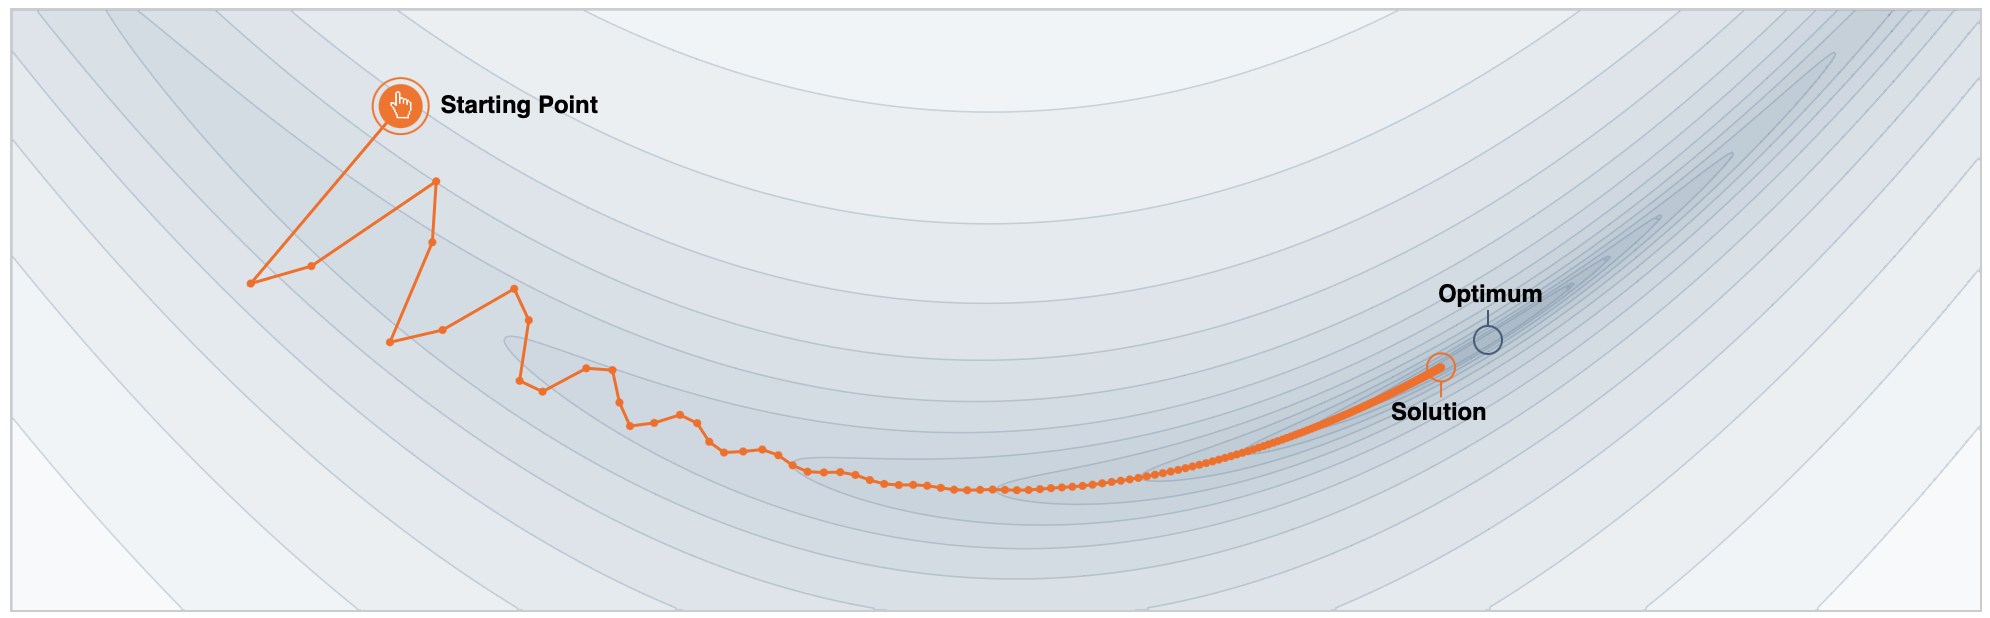
\includegraphics[width=.9\textwidth]{images/distill-momentum.png}
    \caption{Simulation of gradient descent from \href{https://distill.pub/2017/momentum/}{\nolinkurl{https://distill.pub/2017/momentum/}}.}  
\end{figure}

\subsubsection{Gradient descent structure}
Iterative optimization algorithms all follow the same structure:
\begin{description}
    \item[Initialization] We start with a random parameter $\theta_0\in\R^p$. The choice of the initial value is very important in practice, as a good initialization will help our model to converge and reduce overfitting.
    \item[Iteration] The current value of the parameter is updated using a rule of the form
    \begin{equation*}
        \theta_{t+1}=\phi_t(\theta_t,\nabla\L(\theta_t),s_t)
    \end{equation*}
    where $s_t$ is a hidden variable that is also updated at each iteration. The update function, $\phi_t$, might depend on the step $t$ (for instance when using various step sizes). The most basic version of gradient descent is $\theta_{t+1}=\theta_t-\eta\cdot\nabla\L(\theta_t)$, where $\eta$ is the learning rate (or step size).
    \item[Stopping time] The algorithm stops after a certain number $T$ of iterations. This is important in practice and $T$ should be picked carefully to avoid overfitting.
\end{description}

\subsubsection{Difficulties in neural network training}
In practice, training deep neural network can become challenging because of numerous difficulties.
\begin{description}
    \item[Non-convexity] If $\L$ is convex, that is:
    \begin{equation*}
        \forall\theta,\theta'\in\R^p, \quad \L\left(\frac{\theta+\theta'}{2}\right) \leq \frac{\L(\theta)+\L(\theta')}{2}
    \end{equation*}
    the optimization problem is fairly simple. Most theoretical results use this assumption in order to prove the convergence of the algorithm. In practice, this is often not the case, making the optimization problem very hard.
    \item[High dimensionality] The number of parameters $d$ can be huge: for instance, the VGG-16 network, a convolutional neural network trained on the ImageNet dataset, has $p=138\,357\,544$ parameters.
    \item[Access to the gradient] The gradient of $\L$ is often too expensive to compute on the entire dataset. In practice, $\nabla\L(\theta_t)$ is replaced by a stochastic or mini-batch approximation $\tilde{\nabla}_t$. 
\end{description}

\subsubsection{Gradient approximations}
In the following, we will consider that the objective function $\L$ is a loss function between a prediction and a label for one specific example, that is:
\begin{equation*}
    \forall i\in\iset{1}{n}, \quad \L_i(\theta) = \ell(g_\theta(x_i),y_i)
\end{equation*}
Our objective function $\L$ will be the training error:
\begin{equation*}
    \L(\theta) = \frac{1}{n}\sum_{i=1}^n \L_i(\theta) =  \frac{1}{n}\sum_{i=1}^n \ell(g_\theta(x_i),y_i)
\end{equation*}
In the following, $\eta>0$ denotes a \emph{learning rate} (or \emph{step-size}). The following variants of gradient descent are often used:
\begin{description}
    \item[Batch gradient descent] It uses the true gradient:
    \begin{equation*}
        \theta_{t+1} = \theta_t-\eta\cdot\frac{1}{n}\sum_{i=1}^n\nabla\L_i(\theta)
    \end{equation*}
    This approach gives the best possible gradient, but is very expensive if the dataset is large (when $n$ is big).
    \item[Stochastic gradient descent] The gradient is approximated with one random sample
    \begin{equation*}
        \theta_{t+1} = \theta_t-\eta\cdot\L_{i_t}(\theta)
    \end{equation*}
    This approach is very efficient but often instable, since one element might contain noise, making the convergence difficult.
    \item[Mini-batch gradient descent] The gradient is approximated with multiple random samples:
    \begin{equation*}
        \theta_{t+1} = \theta_t-\eta\cdot\frac{1}{b}\sum_{i=1}^b\nabla\L_{i_{b,t}}(\theta)
    \end{equation*} 
    where $b>0$ is the \emph{batch size}. This method is a good tradeoff between speed and convergence, with a parameter $b$ that can be adjusted to obtain the best results.
\end{description}

Keep in mind that the final goal is to reduce the population risk, that is $\E[\ell(g_\theta(X), Y)]$. We need to pay attention to overfitting in addition to using the optimization algorithm to reduce the training error. In this class, we focus specifically on the performance of the optimization algorithm in minimizing the objective function, rather than the model's generalization error. In the next chapters, we will see techniques to avoid overfitting.

\subsection{Convergence analysis}
We aim at providing theoreticla guarantees over the convergence rates of our algorithms. Optimizing non-convex functions is hard in general, but we will make the following assumptions:
\begin{itemize}
    \item The objective function is non-convex but differentiable and $\beta$-smooth, that is:
    \begin{equation*}
        \forall\theta,\theta'\in\R^p, \quad \norm{\nabla\L(\theta)-\nabla\L(\theta')}_2 \leq \beta\cdot\norm{\theta-\theta'}_2
    \end{equation*}
    \item We access unbiased noisy gradients $\tilde{\nabla}_t$, where:
    \begin{equation*}
        \E[\tilde{\nabla}_t] = \nabla\L(\theta_t) \quad \textnormal{and} \quad \V[\tilde{\nabla}_t] \leq\sigma^2
    \end{equation*}
\end{itemize}

\begin{property}[Worst-case convergence to global optimum]
    For any first-order algorithm, there exists a smooth function $\L$ such that its approximation error is at least:
    \begin{equation*}
        \L(\theta_t)-\L(\theta^*) = \Omega(t^{-\frac{1}{d}})
    \end{equation*}
\end{property}
This is prohibitive for large dimensional spaces, since this makes the convergence extremly slow. Therefore, we often choose to restrict ourselves to guarantees for local optima.

\begin{theorem}[Convergence of non-convex SGD to a stationary point]
    Let $\L:\R^p\to\R$ be a smooth function and $\Delta=\L(\theta_0)-\L(\theta^*)$. Then, SGD with step-size:
    \begin{equation*}
        \eta=\min\left(\frac{1}{\beta}, \sqrt{\frac{2\Delta}{T\beta\sigma^2}}\right)
    \end{equation*}
    achieves the error:
    \begin{equation*}
        \E\left[\min_{t\leq T}\norm{\nabla\L(\theta_t)}^2\right] \leq \frac{4\beta\Delta}{T} + \sqrt{\frac{8\beta\Delta\sigma^2}{T}}
    \end{equation*}
    Furthermore,
    \begin{itemize}
        \item without noise, $\eta=\frac{1}{\beta}$ is optimal, and require $O\left(\frac{\beta\Delta}{\epsilon^2}\right)$ iterations for $\norm{\nabla\L(\theta_t)}\leq\epsilon$
        \item with noise, $\eta=O\left(T^{-\frac{1}{2}}\right)$ is optimal, and requires $O\left(\frac{\beta\Delta\sigma^2}{\epsilon^4}\right)$ iterations for $\norm{\nabla\L(\theta_t)}\leq\epsilon$
        \item if $\eta$ is fixed and $\sigma>0$, there is a lower limit in $O\left(\sqrt{\eta\beta}\sigma\right)$ for $\norm{\nabla\L(\theta_t)}$
    \end{itemize}
\end{theorem}

These guarantees prove that GD and SGD converge to a stationary point. Nevertheless, we have no guarantee that this stationary point is actually a local minimum. A local minimum can be defined using second order derivatives: it is both a \textbf{stationary} point, that is $\nabla\L(\theta)=0$, and a \textbf{convexity} point, where the Hessian $H_\L(x)$ is semi-definite positive. The problem is that stationary points can block our algorithm by cancelling the gradient: we are then stuck in saddle points.

An idea to converge towards a local minimum is to add a small noise, allowing the parameter to escape saddle points. When slightly pushed away from the equilibrium by the noise, the parameter will come back to it only is the equilibrium is stable, that is for local minima.

We make the additional assumption that the Hessian $H_\L$ is $\rho$-Lipschitz with respect to the spectral norm. Therefore, with probability at least $1-\delta$, the number of iterations to reach a gradient norm $\norm{\nabla\L(\theta_t)}\leq\epsilon$ and near-convexity $\lambda_1(H_\L(\theta_t))\geq-\sqrt{\rho\epsilon}$ is bounded by:
\begin{equation*}
    O\left(\frac{\beta\Delta}{\epsilon^2}\cdot\log\left(\frac{p\beta\Delta}{\epsilon\delta}\right)^4\right)
\end{equation*}

To conclude:
\begin{itemize}
    \item The loss landscape of deep learning training is non-convex and potentially difficult to optimize
    \item SGD converges to a stationary point in $O(\epsilon^{-4})$ iterations
    \item GD converges to a stationary point in $O(\epsilon^{-2})$ iterations
    \item Adding small noise to GD make it converge to a local minimum in $O(\epsilon^{-2}\log(\epsilon^{-1})^4)$ iterations.
    \item Convergence to a global minimum is prohibitive in high-dimensional spaces. We need at least $\Omega(\epsilon^{-d})$ iterations for smooth functions; we need additional assumptions to ensure fast rates, such as the Polyak-Losasiewicz condition.
\end{itemize}


\subsection{Gradient descent variants}